% To je predloga za poročilo projekta pripredmetu Osnove verjetnosti in
% statistike.
% Originalen avtor predloge je Blaž Zupan.
% Za potrebe OVS je prilagodil Robert Cvitkovič
% To predlogo lahko spremeniš v PDF dokument s pomočjo programa
% pdflatex, ki je del standardne instalacije LaTeX programov.

\documentclass[a4paper,11pt]{article}
\usepackage[utf8]{inputenc}
\usepackage{amsmath, amssymb, amsthm, amsfonts, mathtools}
\usepackage{a4wide}
\usepackage[slovene]{babel}
\usepackage{graphicx}
\usepackage{url}
\usepackage{float}
\usepackage[pdftex,pdfpagelabels,bookmarks,hyperindex,hyperfigures]{hyperref}
% \usepackage{hyperref}
\hypersetup{
pdffitwindow=true,              % window fit to page when opened
pdftitle={Seminarska pri predmetu VIS},       % title
pdfauthor={Matej Kalc},                % author
pdfnewwindow=true,              % links in new window
colorlinks=true,                % false: boxed links; true: colored links
linkcolor=blue,                 % color of internal links
citecolor=blue,                 % color of links to bibliography
filecolor=blue,                 % color of file links
urlcolor=cyan                   % color of external links
}

% \usepackage{tikz}
% \usepackage{pgflibraryshapes}

\usepackage[footnotesize,labelfont=bf,labelsep=period]{caption}
\usepackage{enumerate}
\usepackage{pdfpages}
\usepackage{csvsimple}
\usepackage{graphicx}

\begin{filecontents*}{db.csv}
DR,MED,DPO,DPS,DVO,DVS,OV,MV,PREB,OTO
Austria,44.0,2020-02-25,2020-03-12,2020-03-27,2020-04-23,7029,52,9025715,38809
Belgium,41.4,2020-02-04,2020-03-10,2020-04-11,2020-04-12,32778,4273,11602522,103714
Bulgaria,42.7,2020-03-08,2020-03-12,2020-06-12,2020-06-06,3086,168,6943915,91083
Croatia,43.0,2020-02-25,2020-03-25,2020-04-02,2020-04-20,963,6,4101782,8110
Cyprus,36.8,2020-03-09,2020-03-25,2020-04-02,2020-03-25,320,9,1190007,8468
Czechia,42.1,2020-03-01,2020-03-23,2020-03-27,2020-04-15,2062,9,10715154,36089
Denmark,42.2,2020-02-27,2020-03-15,2020-04-08,2020-04-05,5071,203,5793679,62063
Estonia,42.7,2020-02-27,2020-03-26,2020-03-27,2020-04-03,538,1,1328655,9010
Finland,42.5,2020-01-29,2020-03-21,2020-04-05,2020-04-22,1882,25,5542713,34486
France,41.4,2020-01-24,2020-02-15,2020-04-01,2020-04-04,51477,3514,65283211,233494
Germany,47.1,2020-01-28,2020-03-09,2020-03-20,2020-04-16,18323,45,83951077,595836
Greece,44.5,2020-02-26,2020-03-12,2020-04-22,2020-04-05,2401,121,10420046,58847
Hungary,42.3,2020-03-04,2020-03-15,2020-04-10,2020-04-24,1190,77,9659639,29041
Ireland,36.8,2020-03-01,2020-03-11,2020-04-10,2020-04-26,7393,263,4953657,68922
Italy,45.5,2020-01-29,2020-02-22,2020-03-21,2020-03-28,53578,4827,60465251,239558
Latvia,43.6,2020-03-02,2020-04-04,2020-03-24,2020-04-22,180,0,1883138,8281
Lithuania,43.7,2020-02-28,2020-03-20,2020-04-04,2020-04-12,771,9,2714541,21467
Luxembourg,39.3,2020-03-01,2020-03-13,2020-03-24,2020-04-12,875,8,628614,11189
Malta,41.8,2020-03-07,2020-04-09,2020-04-08,2020-06-02,293,0,441612,14119
Netherlands,42.6,2020-02-27,2020-03-06,2020-03-24,2020-04-08,4749,213,17138553,45825
Poland,40.7,2020-03-05,2020-03-12,2020-06-05,2020-04-25,25048,1117,37850596,1006819
Portugal,42.2,2020-03-02,2020-03-17,2020-04-11,2020-04-04,15472,435,10193282,179542
Romania,41.1,2020-02-26,2020-03-23,2020-04-12,2020-05-01,5990,282,19210031,64385
Slovakia,40.5,2020-03-06,2020-04-07,2020-04-17,2020-04-16,977,8,5461415,42768
Slovenia,44.5,2020-03-04,2020-03-17,2020-03-13,2020-04-06,141,0,2079553,4228
Spain,42.7,2020-01-31,2020-03-04,2020-04-01,2020-06-20,94417,8189,46785134,466271
Sweden,41.2,2020-01-31,2020-03-15,2020-06-23,2020-04-22,58932,5122,10108080,467798
\end{filecontents*}


\begin{filecontents*}{dbIntervalZaupanjaDelezOkuzenih.csv}
Ime drzave,Spodnja meja intervala,Zgornja meja intervala
Austria,0.076\%,0.08\%
Belgium,0.279\%,0.286\%
Bulgaria,0.043\%,0.046\%
Croatia,0.022\%,0.025\%
Cyprus,0.024\%,0.03\%
Czechia,0.018\%,0.02\%
Denmark,0.085\%,0.09\%
Estonia,0.037\%,0.044\%
Finland,0.032\%,0.036\%
France,0.078\%,0.08\%
Germany,0.022\%,0.022\%
Greece,0.022\%,0.024\%
Hungary,0.012\%,0.013\%
Ireland,0.146\%,0.153\%
Italy,0.088\%,0.089\%
Latvia,0.008\%,0.011\%
Lithuania,0.026\%,0.03\%
Luxembourg,0.13\%,0.149\%
Malta,0.059\%,0.075\%
Netherlands,0.027\%,0.029\%
Poland,0.065\%,0.067\%
Portugal,0.149\%,0.154\%
Romania,0.03\%,0.032\%
Slovakia,0.017\%,0.019\%
Slovenia,0.006\%,0.008\%
Spain,0.201\%,0.203\%
Sweden,0.578\%,0.588\%
\end{filecontents*}


\begin{filecontents*}{dbIntervalZaupanjaFatalnost.csv}
Ime drzave,Spodnja meja intervala,Zgornja meja intervala
Austria,0.558\%,0.977\%
Belgium,12.674\%,13.407\%
Bulgaria,4.682\%,6.319\%
Croatia,0.254\%,1.423\%
Cyprus,1.379\%,5.458\%
Czechia,0.213\%,0.859\%
Denmark,3.488\%,4.589\%
Estonia,0.01\%,1.198\%
Finland,0.88\%,1.985\%
France,6.611\%,7.048\%
Germany,0.181\%,0.332\%
Greece,4.215\%,6.011\%
Hungary,5.17\%,8.059\%
Ireland,3.152\%,4.011\%
Italy,8.769\%,9.256\%
Latvia,0\%,2.604\%
Lithuania,0.571\%,2.287\%
Luxembourg,0.426\%,1.869\%
Malta,0\%,1.613\%
Netherlands,3.922\%,5.123\%
Poland,4.209\%,4.724\%
Portugal,2.559\%,3.087\%
Romania,4.192\%,5.283\%
Slovakia,0.381\%,1.675\%
Slovenia,0\%,3.306\%
Spain,8.495\%,8.855\%
Sweden,8.466\%,8.922\%
\end{filecontents*}

\newcommand{\doi}[1]{\href{http://dx.doi.org/#1}{\texttt{doi:#1}}}
\newcommand{\arxiv}[1]{\href{http://arxiv.org/abs/#1}{\texttt{arXiv:#1}}}
\graphicspath{ {./Slike/} }


\title{Covid-19: Potek širjenja do viška prvega vala v Evropski uniji}
\author{Matej Kalc} % (63180368)}
\date{\today}

\begin{document}

\maketitle

\section{Uvod}
\subsection{Motivacija}

% V tem razdelku, 
% ki naj bo kratek in naj obsega en odstavek z do 150 besed, 
% na kratko opišeš, kaj je bil cilj naloge.

\emph{“Koronavirus je hujši kot vojna, kjer je sovražnik še vedno človek, s katerim se še
vedno lahko ukvarjamo, medtem ko je kakršenkoli dogovor s smrtonosnim virusom,
ki ogroža naše preživetje, nemogoč. (...)".} \cite{zucc}\\ \\
Tako je izjavil G. Zuccarini. Lahko bi izjavili, da je Koronavirus tretja svetovna vojna, kjer se neviden sovražnik skriva med ljudmi. Ogroža ljudem življenje, nekaterim pa ga tudi odvzame. Ljudje lahko premagamo nevidnega sovražnika, le če primerno in provočasno ukrepamo s pravim orožjem, kot so samozavest in ukrep človeka. V taki bitki tudi študiji in analize podatkov so dobro orožje proti virusu, saj nam povejo nekaj novega o našem sovražniku. Mogoče eden izmed teh nam bo dal možnost odkritja cepiva proti virusu, toda dokler tega ne najdemo ostaja edina možnost uporaba mask, razkužil in distanca. Zanima me kako so se ljudje odzvali na epidemijo in katere države so bile najboljše in katere najslabše organizirane za preprečevanje okužbe. Ker je epidemija še v teku, bom kot vzorec izbral države Evropske Unije, ker se je v teh epidemija sprožila približno sočasno. 


\subsection{Cilji}
Trdimo lahko, da so vse države v Evropski uniji \cite{eu} preživele prvi val Koronavirusa pred 19.julijem 2020. V seminarski bom analiziral kako se je virus širil po državah evropske unije. Predvsem bom analiziral interval od začetka širjenja do vrhunca prvega vala v vsaki državi, ker je ta interval najzanimivejši, saj se države prvič soočajo s takim virusom. \\
Cilj študija je analiza:
\begin{itemize}
\item{Analiza spremenljivk in}
\item{Korelacijska analiza.}
\end{itemize}
Testiral bom korelacijo med spremenljivkami in izračunal intervale zaupanja, saj podatki niso realni, ker v teh niso vsebovani asimptomatiki.

\subsection{Raziskave o virusu}
Veliko je spletnih strani, ki analizirajo in grafično prikazujejo podatke Covid-a-19. Omenil bom tisto, ki me je motivirala za izdelavo seminarske. \\
Inštitut za zdravstvene meritve in vrednotenje IHME nudi spletno stran o Koronavirus \cite{cvd19IHME}, kjer so grafično prikazani podatki o okuženih, mrtvih, analizah, socialni distanci ipd, ampak najzanimivejše so projekcije v času, ki stran nudi. IHME-ove projekcije COVID-19 so bile razvite kot odziv na zahteve medicinske univerze v Washingtonu in drugih ameriških bolnišničnih sistemov. Napovedi kažejo povpraševanje po storitvah v bolnišnicah, dnevne in kumulativne smrti zaradi COVID-a-19, stopnje okužbe in analizah ter vpliv socialnega distanciranja, ki ga zahteva država.

\subsection{Poglavja}
\begin{enumerate}
\item{Uvod}
\item{Opis virusa in njegovo širjenje}
\item{Podatki}
\item{Izračuni in rezultati}
\item{Zaključki}
\item{Literatura}
\end{enumerate}

\section{Opis virusa in njegovo širjenje}
COVID-19 je nalezljiva bolezen, ki jo povzroča virus SARS-CoV-2. Dihalni virus se širi preko kapljice sline in sluzi okuženih ljudi. Prvi okužen Covid-a-19 je bil zaznan na Kitajskem novembra 2019. Najprej se je dihaln virus širil na Kitajskem, v Hubeju in Wuhanu. Na začetku leta 2020 se je začelo širjenje virusa po celem svetu. 11. marca 2020 je Svetovna zdravstvena organizacija WHO proglasila pandemijo. Iz statističnih podatkov je razvidno, da do vključno 19. julija 2020 je bilo okuženih več kot 14.2 milijonov ljudi v 188 državah, od katerih 600 tisoč je mrtvih in 8.02 milijonov je ozdravelih. Trdimo lahko, da je ta virus leta 2020 močno vplival na države po celem svetu.
\section{Podatki}
Podatki so bili izbrani iz spleta. Podatke, ki bom rabil za statistični študij, so prikazani v spodnji tabeli. \\
\begin{center}
\scalebox{0.8}{
\csvautotabular{db.csv}
}
\end{center}
\paragraph{Legenda:}

\begin{itemize}
\item{DR - Ime države}
\item{MED - Mediana starosti populacije}
\item{DPO - Datum prvega zazanega okuženca}
\item{DPS - Datum prve zaznane smrti}
\item{DVO - Datum vrhunca okuženih v prvem valu}
\item{DVS - Datum vrhunca smrti v prvem valu}
\item{OV - Število okuženih od prve zaznane okužbe do vrhunca okuženih v prvem valu}
\item{MV - Število mrtvih od prve zaznane smrti do vrhunca okuženih v prvem valu}
\item{PREB - Število prebivalcev}
\item{OTO - Število opravljenih testov do vrhunca okužb v prvem valu}
\end{itemize}

V sledečih analizah bom predvsem računal s deleži. Rabil bom sledeče spremenljivke:
\begin{enumerate}
\item{Delež okuženih do vrhunca prvega vala okuženih}
\[D = \frac{100 * \text{št. okuženih}}{\text{št. prebivalcev}}\]
kjer število okuženih je stolpec OV v bazi in število prebivalcev je stolpec PREB v bazi.

\item{Fatalnost do vrhunca prvega vala okuženih}
\[F = \frac{100 * \text{št. mrtvih}}{\text{št. okuženih}}\]
kjer število mrtvih je stolpec MV v bazi in število okuženih je stolpec OV v bazi.

\item{Delež testov do vrhunca prvega vala okuženih}
\[T = \frac{100 * \text{št. opravljenih testov}}{\text{št. prebivalcev}}\]
kjer število opravljenih je stolpec OTO v bazi in število prebivalcev je stolpec PREB v bazi.

\end{enumerate}

\section{Izračuni in rezultati}

\subsection{Analiza spremenljivk}
Za statistični študij bom najprej analiziral spremenljivke, predvsem če so normalne in simetrične Spodnje spremenljivke veljajo le za države evropske unije. Spremenljivke so:
\begin{enumerate}
\item{Mediana starosti}
\item{Število dni do vrhunca prvega vala okuženih}
\item{Število dni do vrhunca prvega vala mrtvih}
\item{Delež okuženih do vrhunca prvega vala okuženih}
\item{Delež mrtvih do vrhunca prvega vala okuženih}
\item{Delež testov do vrhunca prvega vala okuženih}
\end{enumerate}

\subsubsection{Mediana starosti}
Spremenljivka M mediana starosti je stolpec MED v bazi. Naprej lahko prikažemo spremenljivko z histogramom in barplotom.

\begin{figure}[!htb]
   \begin{minipage}{0.5\textwidth}
     \centering
     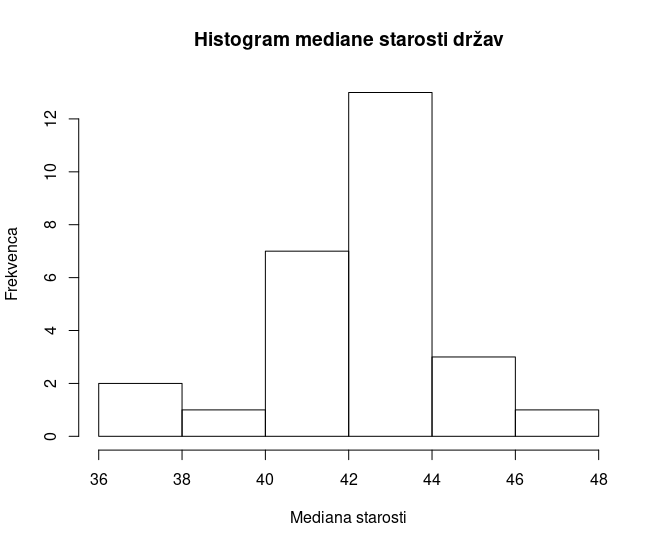
\includegraphics[width=1\linewidth]{histogram_mediane_starosti}
     \caption{Histogram}\label{Fig:Data1}
   \end{minipage}\hfill
   \begin{minipage}{0.5\textwidth}
     \centering
     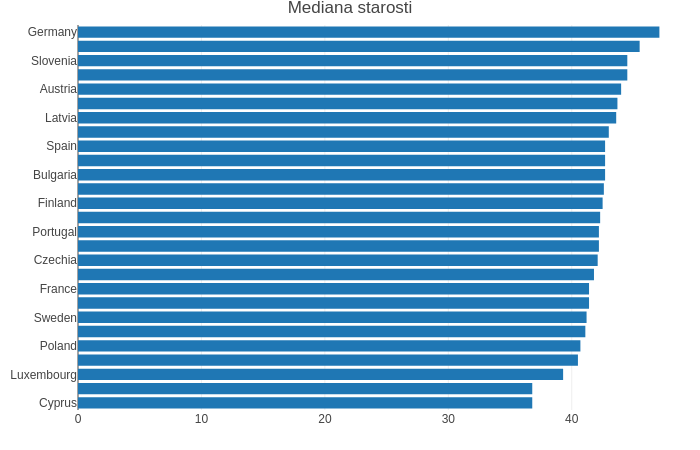
\includegraphics[width=1\linewidth]{barplot_mediane_starosti}
     \caption{Barplot}\label{Fig:Data2}
   \end{minipage}
\end{figure}

Iz histograma lahko sumimo, da je spremenljivka normalna ali simetrična. To lahko preverimo s Shapiro–Wilk testom. Naj bo ničelna hipoteza \(H_0\): spremenljivka je normalna in alternativna hipoteza \(H_1\): spremenljivka ni normalna. Izračunajmoga takole:
\[W = \frac{(\sum_{i = 1}^{n}a_i x_{(i)})^2}{\sum_{i = 1}^{n}(x_i - \overset{\_}{x})^2} = 0.94 \text{ in p} = 0.1218.\]
kjer \(x_{(i)}\) je najmanjša vrednost v vzorcu, \(\overset{\_}{x}\) je povprečje median, \(a_i\) je i-ti element vektorja 0   
\[(a_1,...,a_n) = \frac{m^T V^{-1}}{C}\]
kjer \( C = \left\| V^{-1}m \right\|\) in vektor \(m = (m_1,...,m_n)^T\) je sestavljen iz pričakovanih vrednosti statističnih podatkov o vrstnem redu neodvisnih in identično razporejenih naključnih spremenljivk, vzorčenih iz standardne normalne porazdelitve.
Izberemo 95\% interval zaupanja. \(\alpha\) je 0.05 (1 - 95\%). Če je vrednost p manjša od \(\alpha\), zavržemo \(H_0\). Ker je \(p > \alpha\) (0.1218 \(>\) 0.05), ne moremo zavreči ničelne hipoteze. Iz računa lahko slutimo, da spremenljivka ni normalno porazdeljena. Testiramo lahko, če je spremenljivka M simetrična. Računali bomo s Miao, Gel, and Gastwirth simetričnim testom. V R-ju je to ukaz symmetry.test(X, option = "MGG")\cite{lawstat}, kjer X je poljuben vektor. Naj bo ničelna hipoteza \(H_0\): spremenljivka M je simetrična in alternativna hipoteza \(H_1\): spremenljivka M je asimterična. Za test spremenljivke S dobimo rezultate:
\[\text{Test statistike} = -0.42212 \text{ in p} = 0.684.\]
Tudi tukaj izberemo verjetnost 95\%, tako je \alpha = 0.05. Ker je p vrednost \(> \alpha\) (0.684 \(>\) 0.05) ne moremo zavrnit hipoteze \(H_0\). Zaradi velikega koeficienta p lahko smatramo, da je spremenljivka simetrična.

\subsubsection{Število dni do vrhunca prvega vala okuženih}
Spremenljivka S število dni do vrhunca prvega vala okuženih starosti je razlika v dnevih stolpcev DVO in DPO v bazi. Naprej lahko prikažemo spremenljivko z histogramom in barplotom.

\begin{figure}[!htb]
   \begin{minipage}{0.5\textwidth}
     \centering
     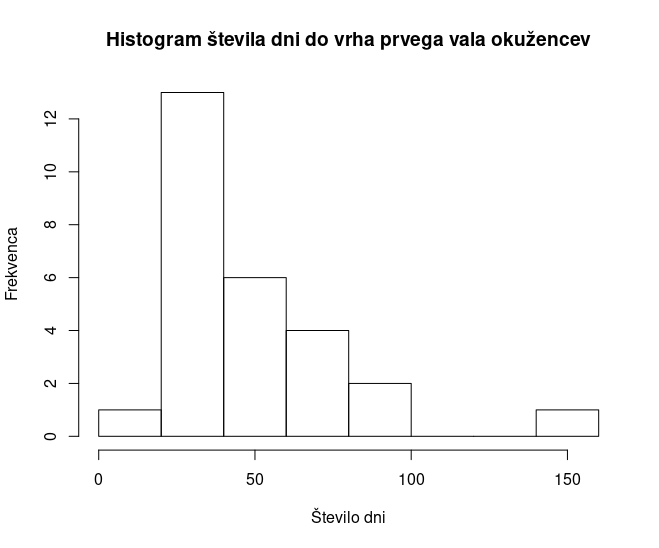
\includegraphics[width=1\linewidth]{histogram_st_dni_do_peaka_okuzencev}
     \caption{Histogram}\label{Fig:Data1}
   \end{minipage}\hfill
   \begin{minipage}{0.5\textwidth}
     \centering
     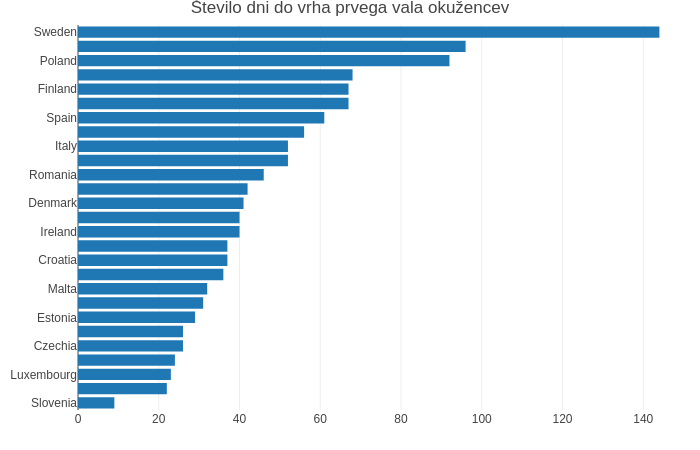
\includegraphics[width=1\linewidth]{barplot_st_dni_do_peaka_okuzencev}
     \caption{Barplot}\label{Fig:Data2}
   \end{minipage}
\end{figure}

Iz histograma ne moremo sumiti, da je spremenljivka normalna ali simetrična. Kot v prejšnji analizi lahko opravimo Shapiro–Wilk test. Naj bo ničelna hipoteza \(H_0\): spremenljivka je normalna in alternativna hipoteza \(H_1\): spremenljivka ni normalna. Enak račun je narejen v paragrafu analize spremenljivke mediane straosti. Izračunajmoga takole:
\[W = \frac{(\sum_{i = 1}^{n}a_i x_{(i)})^2}{\sum_{i = 1}^{n}(x_i - \overset{\_}{x})^2} = 0.85 \text{ in p} = 0.00126. \]
Izberemo 95\% interval zaupanja, kar pomeni, da \(\alpha\) je 0.05 (1 - 95\%). Če je vrednost p manjša od \(\alpha\), zavržemo \(H_0\). Ker je \(p < \alpha\) (0.00126 \(<\) 0.05), zavržemo ničelno hipotezo. Spremenljivka ni normalno porazdeljena, a to še ne pomeni, da ni simetrična. To preverimo s testom simetrije. Računali bomo s Miao, Gel, and Gastwirth simetričnim testom. Naj bo ničelna hipoteza \(H_0\): Spremenljivka S je simetrična in alternativna hipoteza \(H_1\): spremenljivka S je asimterična. Za test spremenljivke S dobimo rezultate:
\[\text{Test statistike} = 2.3151 \text{ in p-value} = 0.052.\]
Tudi tukaj izberemo verjetnost 95\%, tako je \alpha = 0.05. Ker je p vrednost \(> \alpha\) (0.052 \(>\) 0.05) ne moremo zavrnit hipoteze \(H_0\), toda lahko sumimo, da je spremenljivka simetrična, p vrednost zelo majhna.

\subsubsection{Število dni do vrhunca prvega vala mrtvih}
Spremenljivka S število dni do vrhunca prvega vala mrtvih je razlika v dnevih stolpcev DVS in DPS v bazi. Naprej lahko prikažemo spremenljivko z histogramom in barplotom.
\begin{figure}[!htb]
   \begin{minipage}{0.5\textwidth}
     \centering
     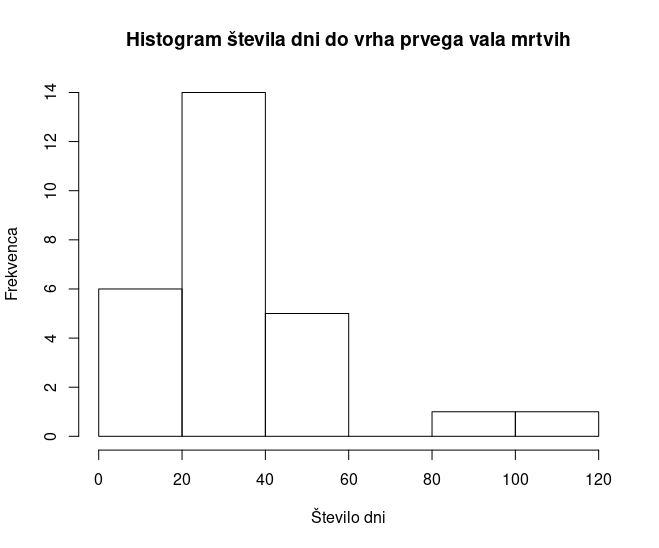
\includegraphics[width=1\linewidth]{histogram_st_dni_do_peaka_mrtvih}
     \caption{Histogram}\label{Fig:Data1}
   \end{minipage}\hfill
   \begin{minipage}{0.5\textwidth}
     \centering
     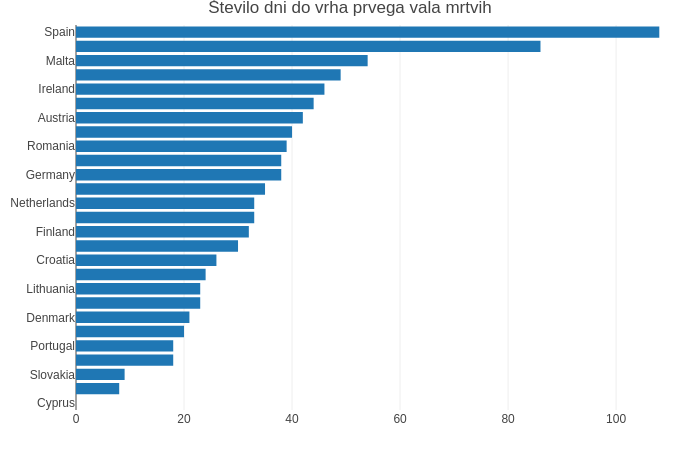
\includegraphics[width=1\linewidth]{barplot_st_dni_do_peaka_mrtvih}
     \caption{Barplot}\label{Fig:Data2}
   \end{minipage}
\end{figure}

Iz histograma ne moremo sumiti, da je spremenljivka normalna ali simetrična. To lahko preverimo s Shapiro–Wilk testom. Naj bo ničelna hipoteza \(H_0\): spremenljivka je normalna in alternativna hipoteza \(H_1\): spremenljivka ni normalna. Enak račun je narejen v paragrafu analize spremenljivke mediane straosti.
\[W = \frac{(\sum_{i = 1}^{n}a_i x_{(i)})^2}{\sum_{i = 1}^{n}(x_i - \overset{\_}{x})^2} = 0.86235 \text{ in p} = 0.00204. \]
Izberemo 95\% interval zaupanja. \(\alpha\) je 0.05 (1 - 95\%). Ker je \(p < \alpha\) (0.00204 \(<\) 0.05), zavržemo ničelno hipotezo. Spremenljivka ni normalno porazdeljena. Menda je simetrična. To preverimo s testom simetrije. Računali bomo s Miao, Gel, and Gastwirth simetričnim testom. Naj bo ničelna hipoteza \(H_0\): spremenljivka S je simetrična in alternativna hipoteza \(H_1\): spremenljivka S je asimterična. Za test spremenljivke S dobimo rezultate:
\[\text{Test statistike} = 0.63107 \text{ in p} =  0.59.\]
Tudi tukaj izberemo verjetnost 95\%, tako je \alpha = 0.05. Ker je p vrednost \(> \alpha\) (0.59 \(>\) 0.05) ne moremo zavrnit hipoteze \(H_0\).

\subsubsection{Delež okuženih do vrhunca prvega vala okuženih}
Naprej lahko prikažemo spremenljivko D delež okuženih do vrhunca prvega vala okuženih (definirano v 3. poglavju) z histogramom in barplotom.

\begin{figure}[!htb]
   \begin{minipage}{0.5\textwidth}
     \centering
     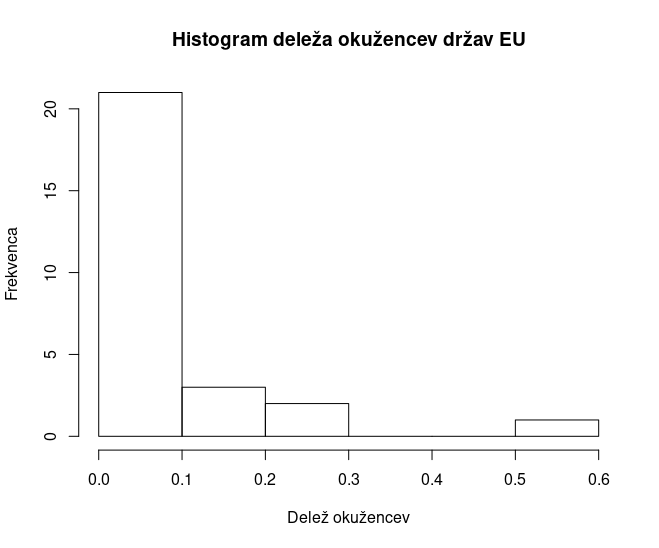
\includegraphics[width=1\linewidth]{histogram_delez_okuzenih}
     \caption{Histogram}\label{Fig:Data1}
   \end{minipage}\hfill
   \begin{minipage}{0.5\textwidth}
     \centering
     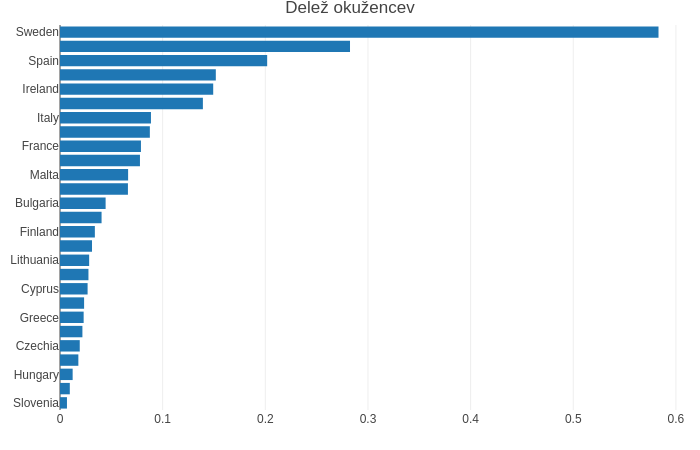
\includegraphics[width=1\linewidth]{barplot_delez_okuzenih}
     \caption{Barplot}\label{Fig:Data2}
   \end{minipage}
\end{figure}
Iz grafov je razvidno, da spremenljivka ni normalna in ni simetrična. To lahko potrdimo s Shapiro–Wilk testom. Naj bo ničelna hipoteza \(H_0\): spremenljivka D je normalna in alternativna hipoteza \(H_1\): spremenljivka D ni normalna. Enak račun je narejen v paragrafu analize spremenljivke mediane straosti. Izračunajmoga takole:
\[W = \frac{(\sum_{i = 1}^{n}a_i x_{(i)})^2}{\sum_{i = 1}^{n}(x_i - \overset{\_}{x})^2} = 0.62339 \text{ in p} = 3.925e-07. \]
Izberemo 95\% interval zaupanja. \(\alpha\) je 0.05 (1 - 95\%). Ker je \(p < \alpha\) (3.925e-07 \(<\) 0.05), zavržemo ničelno hipotezo. Spremenljivka ni normalno porazdeljena, a to še ne pomeni, da ni simetrična. To preverimo s testom simetrije. Naj bo ničelna hipoteza \(H_0\): spremenljivka D je simetrična in alternativna hipoteza \(H_1\): spremenljivka D je asimterična. Za test spremenljivke S dobimo rezultate:
\[\text{Test statistike} = 3.9434 \text{ in p} =  0.002.\]
Tudi tukaj izberemo verjetnost 95\%, tako je \alpha = 0.05. Ker je p vrednost \(< \alpha\) (0.002 \(<\) 0.05) zavrnemo hipotezo \(H_0\). Spremenčjivka D ni normalno porazdeljena in je asimetrična. Delež okužencev je le vzorec, saj v ta delež niso šteti asimpotomatiki. Zaradi tega lahko izračunamo interval zaupanja za vsak delež okuženih. Računamo:
\[\Delta = t_{(1 + \beta) /2}(\infty) \times \sqrt{\frac{p(1 - p)}{n}}\]
kjer n je število prebivalcev države, p je delež okuženih, \(\Delta\) je razmik intervala, \(t_{p}(r)\) je vrednost studentove t-porazdelitve s r stopnjami svobode in p procent zaupanja. Izbrana \(\beta\) je 0.95, kar pomeni, da je \(\alpha = \) 0.05. Državi v i-ti vrstici pripada interval zaupanja \([D_i - \Delta, D_i + \Delta]\), kjer \(D_i\) je delež okuženih za i-to državo. Izračunani intervali so prikazani v spodnji tabeli.
\begin{center}
\csvautotabular{dbIntervalZaupanjaDelezOkuzenih.csv}
\end{center}

\subsubsection{Fatalnost do vrhunca prvega vala okuženih}
Spremenljivko F fatalnost (definirano v 3. pogalvju) prikažemo grafično.

\begin{figure}[!htb]
   \begin{minipage}{0.5\textwidth}
     \centering
     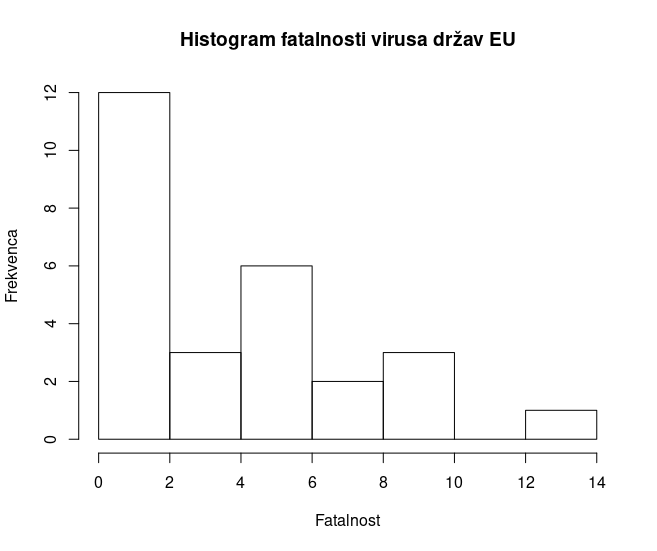
\includegraphics[width=1\linewidth]{histogram_fatalnost}
     \caption{Histogram}\label{Fig:Data1}
   \end{minipage}\hfill
   \begin{minipage}{0.5\textwidth}
     \centering
     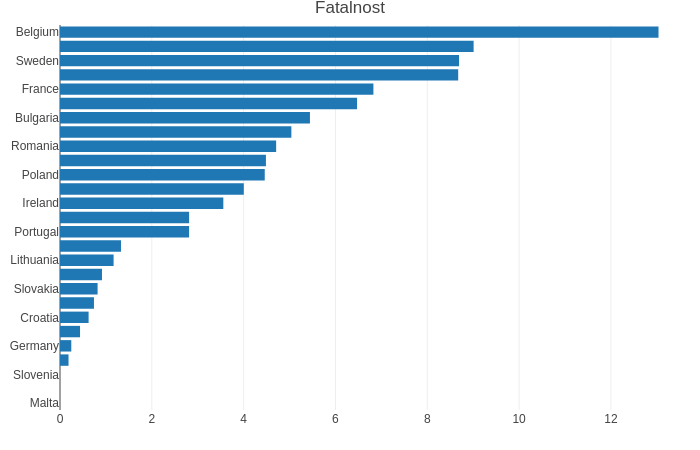
\includegraphics[width=1\linewidth]{barplot_fatalnost}
     \caption{Barplot}\label{Fig:Data2}
   \end{minipage}
\end{figure}
Iz grafov je razvidno, da spremenljivka ni normalna in ni simetrična. To lahko potrdimo s Shapiro–Wilk testom. Naj bo ničelna hipoteza \(H_0\): spremenljivka F je normalna in alternativna hipoteza \(H_1\): spremenljivka F ni normalna. Izračunajmoga takole:
\[W = \frac{(\sum_{i = 1}^{n}a_i x_{(i)})^2}{\sum_{i = 1}^{n}(x_i - \overset{\_}{x})^2} = 0.8851 \text{ in p} = 0.0062. \]
Izberemo 95\% interval zaupanja. \(\alpha\) je 0.05 (1 - 95\%). Ker je \(p < \alpha\) (0.0062 \(<\) 0.05), zavržemo ničelno hipotezo. Spremenljivka ni normalno porazdeljena, a to še ne pomeni, da ni simetrična. To preverimo s testom simetrije. Računali bomo s Miao, Gel, and Gastwirth simetričnim testom. Naj bo ničelna hipoteza \(H_0\): spremenljivka F je simetrična in alternativna hipoteza \(H_1\): spremenljivka F je asimterična. Za test spremenljivke S dobimo rezultate:
\[\text{Test statistike} = 1.5009 \text{ in p} =  0.26.\]
Tudi tukaj izberemo verjetnost 95\%, tako je \alpha = 0.05. Ker je p vrednost \(> \alpha\) (0.26 \(>\) 0.05) ne moremo zavrniti hipotezo \(H_0\). Kot v prejšnji analizu, delež okužencev je le vzorec, saj v ta delež niso šteti asimpotomatiki. Zaradi tega lahko izračunamo interval zaupanja za vsak delež okuženih. Računamo:
\[\Delta = t_{(1 + \beta) /2}(\infty) \times \sqrt{\frac{p(1 - p)}{n}}\]
kjer n je število prebivalcev države, p je delež okuženih, \(\Delta\) je razmik intervala, \(t_{p}(r)\) je vrednost studentove t-porazdelitve s r stopnjami svobode in p procent zaupanja. Izbrana \(\beta\) je 0.95, kar pomeni, da je \(\alpha = \) 0.05. Državi v i-ti vrstici pripada interval zaupanja \([F_i - \Delta, F_i + \Delta]\), kjer \(F_i\) je fatalnost i-te države. Izračunan interval je prikazan v spodnji tabeli.
\begin{center}
\csvautotabular{dbIntervalZaupanjaFatalnost.csv}
\end{center}

\subsubsection{Delež testov do vrhunca prvega vala okuženih}
Spremenljivko T delež testov (definirano v 3. poglavju) prikažemo s histogramom in barplotom.
\begin{figure}[!htb]
   \begin{minipage}{0.5\textwidth}
     \centering
     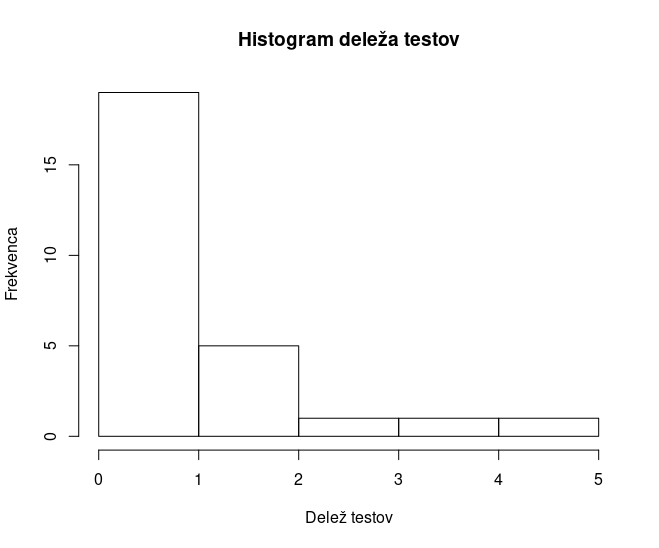
\includegraphics[width=1\linewidth]{histogram_delez_testov}
     \caption{Histogram}\label{Fig:Data1}
   \end{minipage}\hfill
   \begin{minipage}{0.5\textwidth}
     \centering
     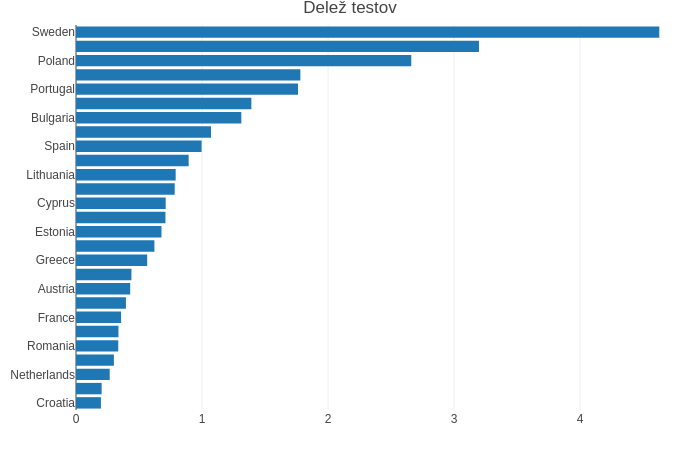
\includegraphics[width=1\linewidth]{barplot_delez_testov}
     \caption{Barplot}\label{Fig:Data2}
   \end{minipage}
\end{figure}
Iz grafov je razvidno, da spremenljivka ni normalna in ni simetrična. To lahko potrdimo s Shapiro–Wilk testom. Naj bo ničelna hipoteza \(H_0\): spremenljivka je normalna in alternativna hipoteza \(H_1\): spremenljivka ni normalna. Računamo:
\[W = \frac{(\sum_{i = 1}^{n}a_i x_{(i)})^2}{\sum_{i = 1}^{n}(x_i - \overset{\_}{x})^2} = 0.73562 \text{ in p} = 1.264e-05. \]
Izberemo 95\% interval zaupanja. \(\alpha\) je 0.05 (1 - 95\%). Ker je \(p < \alpha\) (1.264e-05 \(<\) 0.05), zavržemo ničelno hipotezo. Spremenljivka ni normalno porazdeljena, a to še ne pomeni, da ni simetrična. To preverimo s testom simetrije. Računali bomo s Miao, Gel, and Gastwirth simetričnim testom. Naj bo ničelna hipoteza \(H_0\): spremenljivka T je simetrična in alternativna hipoteza \(H_1\): spremenljivka T je asimterična. Za test spremenljivke S dobimo rezultate:
\[\text{Test statistike} = 2.8186 \text{ in p-value} =  0.018.\]
Tudi tukaj izberemo verjetnost 95\%, tako je \alpha = 0.05. Ker je p vrednost \(< \alpha\) (0.018 \(<\) 0.05) zavrnemo ničelno hipotezo \(H_0\). Spremenčjivka T ni normalno porazdeljena in je asimetrična.

\subsection{Korelacijska analiza}
Korelacijsko analizo bom razdelil na tri dele in sicer:
\begin{enumerate}
\item{Mediana starosti}
\item{Delež testov starosti}
\item{Število dni do vrha prvega vala okuženih}
\end{enumerate}

\subsubsection{Mediana starosti}
Zanima me kako je mediana starosti vplivala na druge spremenljivke in sicer na število dni do vrhunca prvega vala okuženih, število dni do vrhunca prvega vala mrtvih, delež okuženih do vrhunca prvega vala okuženih, delež mrtvih do vrhunca prvega vala okuženih. Naj bo spremenljivka M mediana starosti (stolpec MED v bazi), spremenljivka ŠO število dni do vrhunca prvega vala okuženih, spremenljivka ŠM število dni do vrhunca prvega vala mrtvih, spremenljivka D delež okuženih (definirana v 3. poglavju) in spremenljivka F fatalnost (definirana v 3. poglavju). Podatke navedenih spremenljivk lahkjo prikažemo z razsvenim grafom.

\begin{figure}
    \centering
    \subfigure{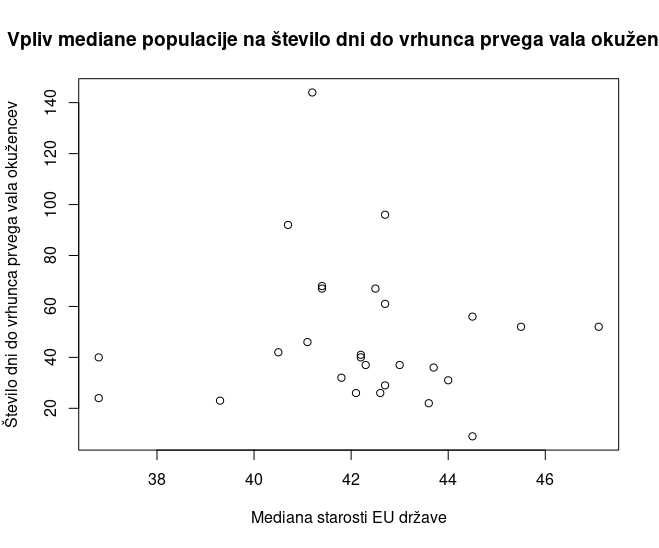
\includegraphics[width=0.4\textwidth]{vpliv_med_populacije_na_st_dni_do_peaka_okuezenih}}
    \subfigure{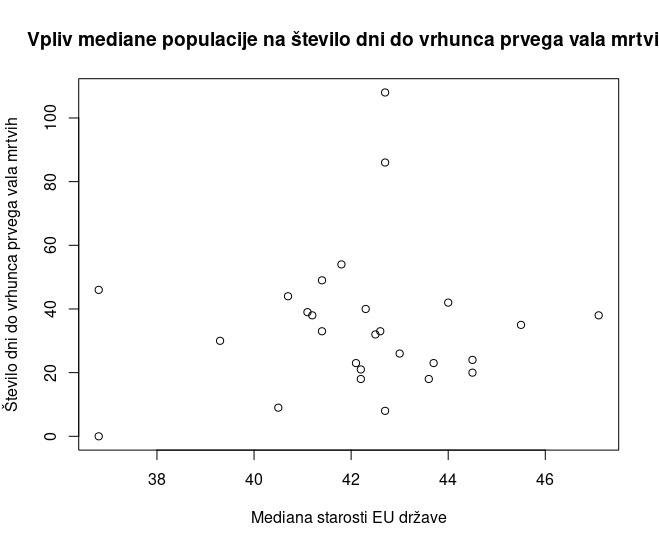
\includegraphics[width=0.4\textwidth]{vpliv_med_pop_na_st_dni_do_peaka_mrtvih}} 
    \subfigure{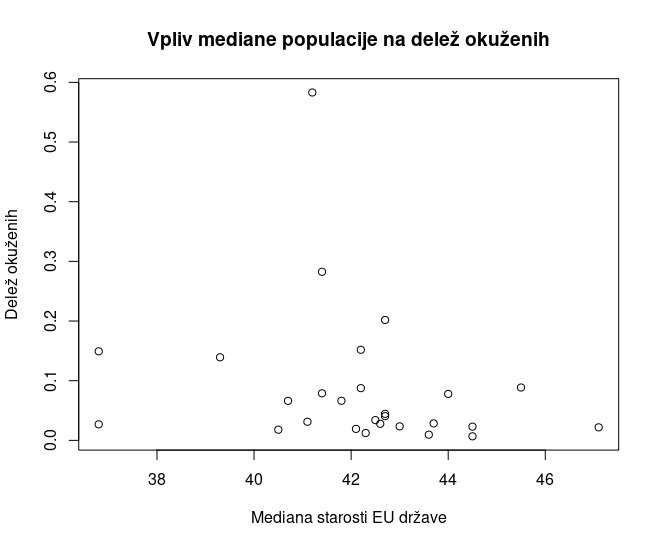
\includegraphics[width=0.4\textwidth]{vpliv_med_pop_na_delez_okuzencev}}
    \subfigure{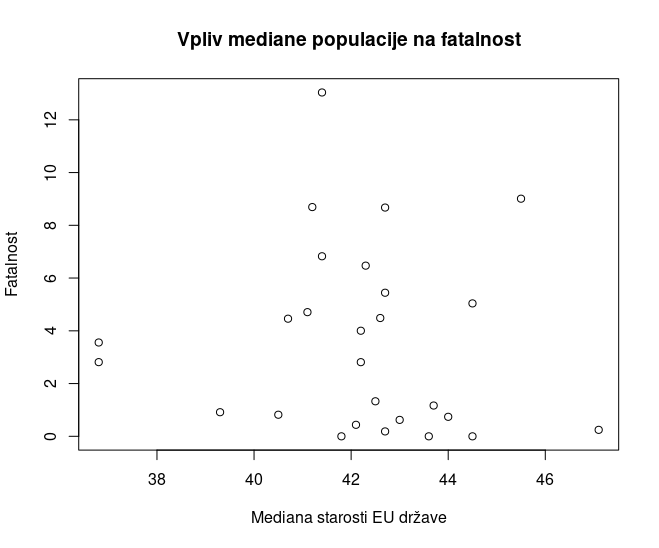
\includegraphics[width=0.4\textwidth]{vpliv_med_pop_na_fatalnost}}
\end{figure}
Velja, da v nobenem diagramu uspemo zaznati nek trend, toda to še ne pomeni, da so si pari spremenljivk neodvisni. Vsako korelacijo lahko izmerimo z Pearsonovim koeficientom korelacije:
\[r_1 = \frac{Cov(M,ŠO)}{\sigma_{M} \sigma_{ŠO}} = -0.0258 r_2 = \frac{Cov(M,ŠM)}{\sigma_{M} \sigma_{ŠM}} = 0.0902\]
\[r_3 = \frac{Cov(M,D)}{\sigma_{M} \sigma_{D}} = -0.2203 r_4 = \frac{Cov(M,F)}{\sigma_{M} \sigma_{F}} = -0.0845\]

kjer so \(\sigma_{M}\) standardni odklon spremenljivke M, \(\sigma_{ŠO}\) standardni odklon spremenljivke ŠO, \(\sigma_{ŠM}\) standardni odklon spremenljivke ŠM, \(\sigma_{D}\) standardni odklon spremenljivke D in \(\sigma_{F}\) standardni odklon spremenljivke F. Noben koeficient ni dovolj velik, da bi lahko smatrali, da obstaja močna povezanost med spremenljivkima. Pravzaprav ker je vsak koeficient tako blizu ničle lahko smatramo, da sta spremenljivka M mediana starosti ne vpliva na ostale izbrane spremenljivke, to pa še ni gotovo. Ker je število okuženecv le vzorec, ker niso šteti asimptomatiki, lahko izračunamo interval zaupanja za zgornje korelacijske koeficiente. V R-ju lahko izračunamo 95\% interval zaupanja z ukazom cor.test(M,X, method = "pearson"), kjer X je izbrana spremenljivka. Izračunani intervali zaupanjaa so:
\[[r_1 - \Delta_1, r_1 + \Delta_1] = [-0.4019, 0.3577]\]
\[[r_2 - \Delta_2, r_2 + \Delta_2] = [-0.3001382, 0.4545977]\]
\[[r_3 - \Delta_3, r_3+ \Delta_3] = [-0.5539, 0.1743]\]
\[[r_4 - \Delta_4, r_4 + \Delta_4] = [-0.45, 0.3053]\]
Da bi bila spremenljivka M v korelaciji z neko drugo izbrano spremenljivko, bi moral biti koeficient korelacije močno pozitiven oziroma večji od 0.7 ali močno negativen oziroma manjši od -0.7. Nobena vrednost v zgornejih intervalih, ne zadošča pogoju zaradi tega lahko smatramo z verjetnostjo 95\%, da sta spremenljivka M ne vpliva nobeno drugo izbrano spremenljivko.

\subsubsection{Delež testov}

Zanima me kako je delež testov vpliva na druge spremenljivke in sicer na delež okuženih do vrhunca prvega vala okuženi in na delež mrtvih do vrhunca prvega vala okuženih. Naj bojo spremenljivka T delež testov, spremenljivka D delež okuženih in spremenljivka F fatalnost (vse tri definirane v 3. poglavju). Podatke navedenih spremenljivk lahko prikažemo z razsvenim grafom.

\begin{figure}
    \centering
    \subfigure{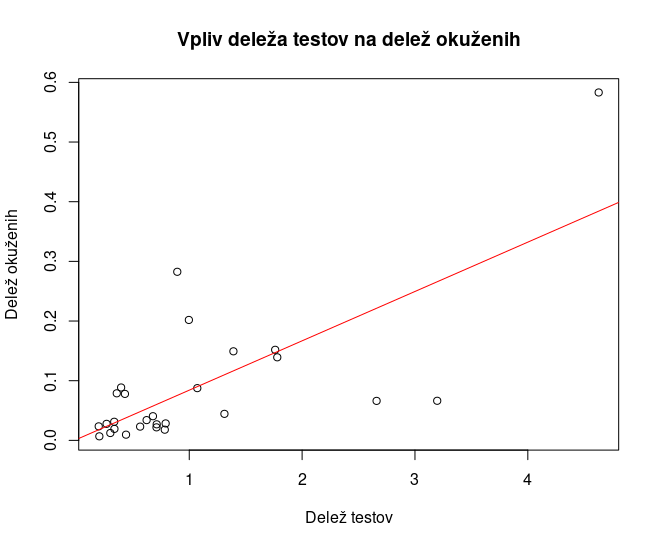
\includegraphics[width=0.4\textwidth]{vpliv_deleza_testov_na_delez_okuzenih}}
    \subfigure{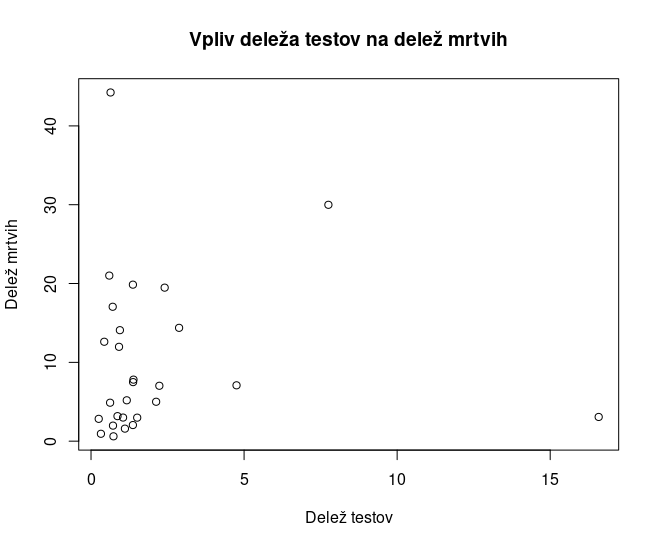
\includegraphics[width=0.4\textwidth]{vpliv_delez_testov_na_delez_mrtvih}} 
\end{figure}

Iz levega grafa lahko zaznamo nek trend med spremenljivkama T in D. Koeficient korelacije parov spremenljivk lahko izračunamo s Pearsonovim koeficientom korelacije:

\[r_1 = \frac{Cov(T,D)}{\sigma_{T} \sigma_{D}} = 0.7131\]
\[r_2 = \frac{Cov(T,F)}{\sigma_{T} \sigma_{F}} = 0.1596\]

kjer so \(\sigma_{M}\) standardni odklon spremenljivke M, \(\sigma_{F}\) standardni odklon spremenljivke F in \(\sigma_{D}\) standardni odklon spremenljivke D. Koeficient \(r_1\)je dovolj velik, da bi lahko smatrali, da obstaja močna povezanost med spremenljivkima T in D. Lahko trdimo, da spremenljivki sta si odvisni. Enako ne velja za par spremenljivk T in F, kjer korelacijski koeficient \(r_2\) je premajhen, da bi lahko sumili močno povezanost.

Kot v razdelku 4.2.1 je število okuženecv le vzorec, saj niso šteti asimptomatiki zaradiu tega lahko izračunamo 95\% interval zaupanja za korelacijski koeficient. 
\[[r_1 - \Delta_1, r_1 + \Delta_1] = [0.4568, 0.86]\]
\[[r_2 - \Delta_2, r_2 + \Delta_2] = [-0.45, 0.3053]\]

Da bi bila spremenljivka T v korelaciji z neko drugo izbrano spremenljivko, bi moral biti koeficient korelacije močno pozitiven oziroma večji od 0.7 ali močno negativen oziroma manjši od -0.7. Prvi interval zadošča temu pogoju, saj \(r_1\) je večji od 0.7. Drugi interval pa nam pove, da ne obstaja z verjetnostjo 95\% močna povezanost med spremenljivkima T in F.

\subsubsection{Število dni do vrha prvega vala okuženih}

Zanima me kako je število dni do vrha prvega vala okuženih vpliva na druge spremenljivke in sicer na delež okuženih do vrhunca prvega vala okuženi in na delež mrtvih do vrhunca prvega vala okuženih. Naj bojo spremenljivka Š število dni do vrhunca prvega vala okuženih starosti (razlika v dnevih stolpcev DVO in DPO v bazi), spremenljivka D delež okuženih in spremenljivka F fatalnost (zadnje dve sta definirane v 3. poglavju). Podatke navedenih spremenljivk lahko prikažemo z razsvenimi diagrami.

\begin{figure}
    \centering
    \subfigure{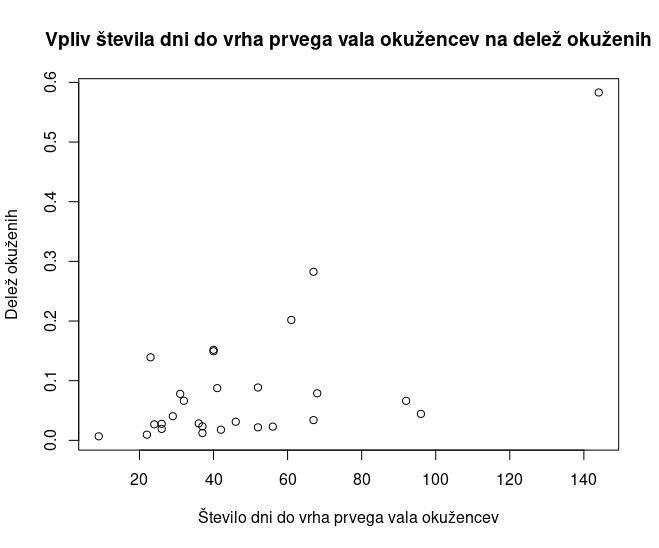
\includegraphics[width=0.4\textwidth]{vpliv_stevila_dni_do_peaka_okuzencev_na_delez_okuzenih}}
    \subfigure{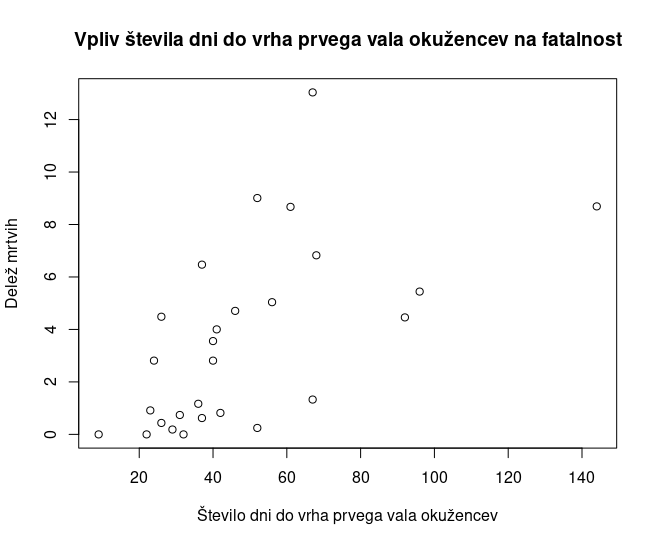
\includegraphics[width=0.4\textwidth]{vpliv_stevila_dni_do_peaka_okuzencev_na_fatalnost}} 
\end{figure}
Iz grafa lahko zaznamo nek trend med spremenljivkama Š in D. Podobno ne velja za desni diagram. Kot v zgornjih razdelkih izračunamo Pearsonov koeficient korelacije:

\[r_1 = \frac{Cov(Š,D)}{\sigma_{Š} \sigma_{D}} = 0.6755\]
\[r_2 = \frac{Cov(Š,F)}{\sigma_{Š} \sigma_{F}} = 0.5856\]

kjer so \(\sigma_{Š}\) standardni odklon spremenljivke Š, \(\sigma_{F}\) standardni odklon spremenljivke F in \(\sigma_{D}\) standardni odklon spremenljivke D. Trdimo lahko, da obstaja linearna povezanost med spremenljivko Š in D, saj njihov korelacijski koeficient se bliža vrednosti 0.7. 
Ker je število okuženecv le vzorec, izračunamo 95\% interval zaupanja za korelacijski koeficient. Izračunani intervali zaupanja so:
\[[r_1 - \Delta_1, r_1 + \Delta_1] = [0.3976, 0.8399]\]
\[[r_2 - \Delta_2, r_2 + \Delta_2] = [0.2644, 0.7898]\]


\section{Zaključki}\
Iz analize spremenljivk lahko trdimo, da spremenljivke število dni do vrhunca prvega vala okuženih, števila dni do vrhunca prvega vala mrtvih, delež okuženih, delež mrtvih in delež testov niso normalno porazdeljene. Sklepamo lahko, da na te spremenljivke vplivajo drugi različni faktorji, kot je čas, ki je potrebovala posamezna država za regulacije (maske, rokavice in socialno distanciranje), saj vsaka država je ukrepala poljubno. \\
Iz korelacijske analiza lahko smatramo, da spremenljivka mediane starosti ni lineareno korelirana z številom dni do vrhunca prvega vala okuženih, številom dni do vrhunca prvega vala mrtvih, deležom okuženih do vrhunca prvega vala okuženih, deležom mrtvih do vrhunca prvega vala okuženih. Noben koeficient korelacije ni pozitivno močen ali negativno močen, pravzaprav so vsi zelo blizu ničli, razen za delež okuženih. Podobno velja za izračunane intervale zaupanja zaradi tega se sluti, da spremenljivka mediana starosti ne vpliva na ostale izbrane spremenljivke. \\
Korelacijska analiza deleža testov in drugih izbranih spremenljivk je privedla do zanimivih rezultatov. Izkaže se, da je spremenljivka deleža testov linearno povezana z deležom okuženih, saj če država opravi več testov lahko zazna več okužencev in veča zaznani delež okuženih. Enako se ne izkaže za fatalnost virusa. Na fatalnost vplivajo tudi drugi faktorji, kot so zmogljivost bolnišnic in če je bolnik imel še druge bolezni. \\
Korelacijska analiza števila dni do vrha prvega vala okuženih in drugih izbranih spremenljivk je tudi privedla do zanimivih rezultatov. Število dni do vrha prvega vala okuženih in delež okuženih sta si skoraj linearno povezani. Lahko zaklučimo, da je smiselno, da obstaja neka povezanost med spremenljivkima, saj v večjem številu dni se lahko zazna in zboli več okuženih ljudi. Podobno velja za spremenljivki število dni do vrha prvega vala okuženih in fatalnost, kjer linearna korelacija obstaj, toda ni tako visoka, da bi jo smatrali za močno. Se pravi, ne moremo trditi, da sta ti dve spremenljivki odvisni. Smatramo lahko, da daljša je prva polovica prvega vala okuženih več bo okuženih in posledično več bo mrtvih. \\
Globalno gledano se je izkazalo, da mediana starosti populacije ni igrala tako pomebne vloge v širjenjem virusa v prvi polovici prvega vala okuženih. Obratno velja za delež testov in število dni do vrha prvega vala okuženih. Za katerih velja, da sta pozitvno linearno povezani z deležom okuženih. Iz tega sledi, da višje je število opravljenih testov višje je število zaznanih okuženih in višje je število dni do vrha prvega vala okuženih višji je delež okuženih.

\section{Literatura}

\begin{thebibliography}{9}

\bibitem{zucc} 
Citat - Zuccarini,
\\\texttt{https://www.frasicelebri.it/frase/zuccarini-giuseppe-coronavirus-e-peggio-di-una-gue/}

\bibitem{medageWiki} 
List of countries by median age - Wikipedia,
\\\texttt{https://en.wikipedia.org/wiki/List\_of\_countries\_by\_median\_age}

\bibitem{eu} 
List of EU countries - Wikipedia,
\\\texttt{https://en.wikipedia.org/wiki/European\_Union}


\bibitem{popEU} 
List of European countries by population - Wikipedia,
\\\texttt{https://en.wikipedia.org/wiki/List\_of\_European\_countries\_by\_population}


\bibitem{cvd19IHME} 
Covid-19 - IHME,
\\\texttt{https://covid19.healthdata.org/}


\bibitem{cvd19WHO} 
Covid-19 - WHO,
\\\texttt{https://covid19.who.int/info}


\bibitem{github} 
Github repository - Matej Kalc,
\\\texttt{https://github.com/KalcMatej99/Seminarska-VS-Covid-19}


\bibitem{marty} 
Pandemija koronavirusa: biološki, mikrobiološki in kemijski izsledki te okužbe - Martina Lizza,
\\\texttt{https://drive.google.com/file/d/1KwhX7zzNJ0x5NnlzdY\_DXD\_-JdxXiGNj/view?usp=sharing}

\bibitem{cvd19Wiki} 
Covid-19 - Wikipedia
\\\texttt{https://en.wikipedia.org/wiki/Coronavirus\_disease\_2019}

\bibitem{lawstat} 
Lawstat R package - Vyacheslav Lyubchich
\\\texttt{https://www.rdocumentation.org/packages/lawstat/versions/3.4}



\end{thebibliography}

\end{document}
